\documentclass[twocolumn,10pt]{article}
\usepackage[utf8]{inputenc}
\usepackage[T1]{fontenc}
\usepackage{mathptmx}
\usepackage[margin=0.6in,top=0.55in,bottom=0.6in]{geometry}
\usepackage{amsmath,amssymb}
\usepackage{booktabs}
\usepackage{graphicx}
\usepackage{microtype}
\usepackage{cite}
\usepackage{enumitem}
\usepackage{xcolor}
\usepackage{titlesec}
\usepackage{caption}
\usepackage[colorlinks=true,linkcolor=blue,citecolor=blue,urlcolor=blue]{hyperref}

% Tight spacing for the 2-page limit
\titleformat{\section}{\normalfont\large\bfseries}{\thesection}{0.5em}{}
\titleformat{\subsection}{\normalfont\normalsize\bfseries}{\thesubsection}{0.5em}{}
\titlespacing{\section}{0pt}{4pt plus 1pt minus 1pt}{2pt plus 1pt minus 1pt}
\titlespacing{\subsection}{0pt}{3pt plus 1pt minus 1pt}{1pt plus 1pt minus 1pt}
\setlength{\parskip}{1pt plus 0.5pt minus 0.5pt}
\setlength{\parindent}{1em}
\setlength{\columnsep}{0.22in}
\setlength{\textfloatsep}{5pt plus 2pt minus 2pt}
\setlength{\floatsep}{4pt plus 2pt minus 2pt}
\setlength{\dbltextfloatsep}{5pt plus 2pt minus 2pt}
\captionsetup{font=small,skip=2pt}
\setlist{leftmargin=*,itemsep=0pt,topsep=1pt,partopsep=0pt,parsep=0pt}

\begin{document}

\twocolumn[{%
\begin{center}
  {\Large\bfseries RL for Adaptive Cache Replacement Under Changing Workloads}\\[3pt]
  \textbf{Lakshya Jain} (B23CS1032, \texttt{b23cs1032@iitj.ac.in}) \quad
  \textbf{Ripu Daman Singh} (B23CS1057, \texttt{b23cs1057@iitj.ac.in})\\
  Department of Computer Science and Engineering, IIT Jodhpur\\
  \textbf{GitHub:} \url{https://github.com/Damanish/adaptive_cache_replacement_rl}\\
  \textbf{Interactive results:} \url{https://damanish.github.io/adaptive_cache_replacement_rl/}\\[3pt]
  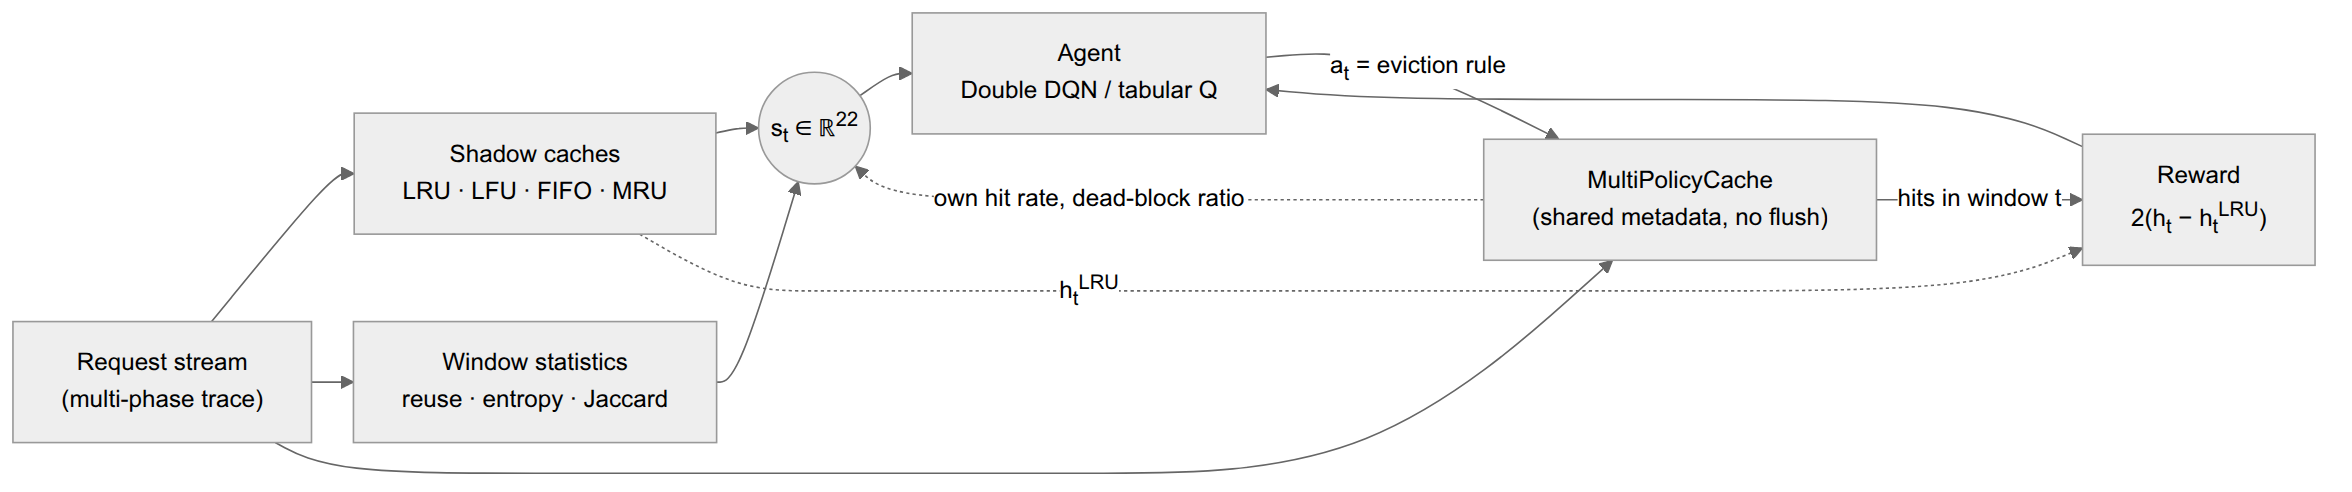
\includegraphics[width=0.93\textwidth]{figures/system_overview.png}
  \captionof{figure}{System overview. Once per window of $W{=}100$ requests the agent observes causal
  statistics of the past stream and picks the eviction rule used by every miss in the next window.
  The relative reward subtracts the action-independent shadow-LRU hit rate.}
  \label{fig:system}
  \vspace{4pt}
\end{center}}]

\noindent\textbf{Abstract---}No single cache replacement policy is best for all access patterns:
LRU collapses on scans and loops, LFU on shifting working sets. We cast \emph{policy selection} as
a reinforcement-learning problem: every $W$ requests an agent chooses which eviction rule
(LRU/LFU/FIFO, optionally MRU) a shared-metadata cache applies next. On 20 held-out
multi-phase traces, Double DQN beats every non-clairvoyant baseline including ARC
(+0.38\,pp, 18/20 traces, $p{<}10^{-3}$); with MRU added it reaches 63.6\% hit rate
(ARC 57.1\%, Belady 68.6\%) and cuts modelled AMAT by 19\% versus LRU.

\section{Problem and Related Work}
Adaptive heuristics such as ARC~\cite{megiddo2003arc}, LIRS~\cite{jiang2002lirs} and set-dueling
DIP~\cite{qureshi2007dip} hard-code \emph{how} to adapt. Learned approaches predict
per cache line, imitating Belady's MIN (Hawkeye~\cite{jain2016hawkeye},
Parrot~\cite{liu2020parrot}) or distilling an RL agent into a hardware policy
(RLR~\cite{sethumurugan2021rlr}). Closest to us, LeCaR~\cite{vietri2018lecar} and
CACHEUS~\cite{rodriguez2021cacheus} weight expert policies online by regret minimisation. We instead learn an \emph{offline-trained,
state-conditioned} selector over expert policies: one cheap inference per window instead of per
request, and the agent can exploit cues (scan stride, loop reuse distance) that regret weights see
only after losses accumulate.

\textbf{Workloads.} Traces concatenate 6 random phases (3--8k requests each, disjoint key
ranges) from five regimes, each favouring a different policy: \emph{zipf} ($\alpha\!\in\![0.9,1.2]$,
frequency), \emph{drift} (hot set of $0.6$--$0.9C$ that relocates every $3$--$6C$ requests,
recency), \emph{scan} (hot set plus one-shot sequential runs), \emph{stack} (LRU stack-distance
model) and \emph{loop} (cyclic sweep over $1.1$--$1.5C$ blocks plus a small hot set).
Train/val/test use disjoint seeds (64/8/20 traces); $C{=}W{=}100$.

\section{RL Formulation}
An episode is one trace; step $t$ covers requests $[tW,(t{+}1)W)$, a semi-MDP over macro-actions.

\textbf{State $\mathcal{S}\subset\mathbb{R}^{22}$} (identical layout for 3 and 4 actions; computed only
from windows $<t$, verified by a causality test): (i) hit rates of four \emph{shadow caches}
running fixed LRU/LFU/FIFO/MRU on the same stream, last window and EMA ($\beta{=}0.8$) (8 dims);
(ii) stream statistics of the last window (7 dims): unique-key ratio, sequential-stride ratio
$\Pr[k_i{=}k_{i-1}{+}1]$, first-reference ratio, reuse-interval buckets $\Delta\!\le\!C$ and
$C\!<\!\Delta\!\le\!4C$, normalised popularity entropy $-\sum p_i\ln p_i/\ln W$, and key-set Jaccard
overlap with the previous window (a phase-change cue); (iii) agent state (7 dims): own hit rate and
its EMA, fraction of resident blocks never re-referenced, one-hot previous action (4 slots).

\textbf{Action $\mathcal{A}$} (discrete): $\{$LRU, LFU, FIFO$\}$, or $\{$LRU, LFU, FIFO, MRU$\}$
in the extended setting. The action fixes the victim rule for all misses in window $t$.

\textbf{Reward $\mathcal{R}$.} Raw hit rate swings with phase difficulty (Belady reaches only
0.29 on scans but 0.83 on drift), inflating TD-target variance. We use a relative reward
\begin{equation}
  r_t = 2\,(h_t - h^{\text{LRU}}_t) - \lambda\,\mathbf{1}[a_t\neq a_{t-1}],
\end{equation}
where $h^{\text{LRU}}_t$ is the shadow-LRU hit rate of the \emph{same} window. Because the request
stream is exogenous, this term is independent of the agent's actions: it shifts all action values
of a state equally and leaves the greedy policy unchanged. We use $\lambda{=}0$; a hit/miss reward
$2h_t{-}1$ and a latency reward $-\text{AMAT}_t/L_{\text{miss}}$ are also implemented.

\textbf{Environment.} \texttt{MultiPolicyCache} keeps last-access time, insertion time and an
exponentially aged frequency $f_i\leftarrow f_i\,2^{-(t-t_{\text{last}})/H}{+}1$ ($H{=}10C$) for
every slot, so a policy switch only changes the victim rule and never flushes the cache. Aging stops
LFU from keeping blocks that were hot in an earlier phase.

\textbf{Algorithms.} \emph{Tabular Q-learning} on a discretised state
(best shadow policy $\times$ its margin $\times$ own-hit-rate bin $\times$ previous action $\times$
Jaccard flag; 216/384 states), $\alpha{=}0.1$, 300 episodes. \emph{Double DQN}~\cite{vanhasselt2016deep}:
MLP $22\!\to\!128\!\to\!128\!\to\!|\mathcal{A}|$, Huber loss, Adam ($5{\times}10^{-4}$), replay 50k,
Polyak $\tau{=}0.01$, 150 episodes ($\approx$49k steps). Both use $\gamma{=}0.9$, linear
$\epsilon$-decay $1\!\to\!0.03$ over 60\% of training, and keep the checkpoint with the best
validation hit rate (Fig.~\ref{fig:training}).

\textbf{Baselines.} Fixed LRU/LFU/FIFO/MRU; Random; FTL (pick last window's best shadow policy,
i.e.\ the same information without learning); Phase-Oracle (best \emph{single} fixed policy for each
true phase, chosen in hindsight); ARC~\cite{megiddo2003arc}; Belady's MIN~\cite{belady1966study}
(offline optimum). ARC and MIN were fuzz-tested against invariants and brute force.

\section{Results}
\begin{table}[t]
\centering\small
\caption{Held-out test traces ($C{=}100$, 20 traces). AMAT with $L_{\text{hit}}{=}1$,
$L_{\text{miss}}{=}100$. Post-chg.: mean hit rate over 10 windows after each phase change.
Random/FTL/Phase-Oracle use 3 actions; Fixed-MRU is from the 4-action run.}
\label{tab:main}
\setlength{\tabcolsep}{4pt}
\begin{tabular}{lcccc}
\toprule
Method & Hit rate & $\pm$std & AMAT & Post-chg. \\
\midrule
Fixed-LRU & 54.71 & .074 & 45.84 & 53.51 \\
Fixed-LFU (aged) & 33.14 & .040 & 67.19 & 33.76 \\
Fixed-FIFO & 52.27 & .073 & 48.26 & 51.28 \\
Fixed-MRU & \phantom{0}4.32 & .028 & 95.73 & \phantom{0}2.01 \\
Random & 50.88 & .068 & 49.63 & 50.80 \\
FTL & 55.73 & .075 & 44.83 & 53.41 \\
Phase-Oracle & 56.79 & .067 & 43.77 & 52.54 \\
ARC~\cite{megiddo2003arc} & 57.11 & .066 & 43.46 & 54.20 \\
\midrule
Q-learning (3 act.) & 56.79 & .070 & 43.78 & 53.75 \\
DQN (3 act.) & \textbf{57.50} & .068 & \textbf{43.08} & \textbf{54.49} \\
\midrule
Q-learning (+MRU) & 60.09 & .070 & 40.51 & 54.49 \\
DQN (+MRU) & \textbf{63.58} & .066 & \textbf{37.06} & \textbf{58.03} \\
\midrule
Belady MIN (offline) & 68.63 & .072 & 32.06 & 66.19 \\
\bottomrule
\end{tabular}
\end{table}

\begin{figure}[t]
  \centering
  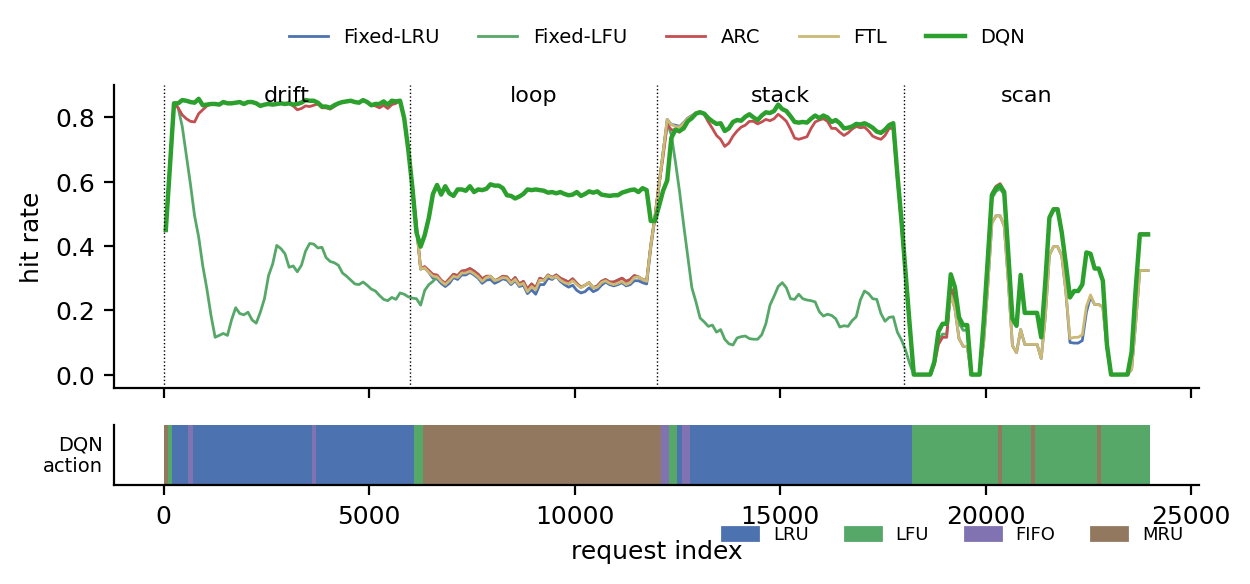
\includegraphics[width=\columnwidth]{figures/timeline_drift_loop_stack_a4.png}
  \caption{Drift$\to$loop$\to$stack$\to$scan scenario (+MRU). DQN switches to MRU when the loop
  starts (phase mean 0.55 vs.\ 0.29--0.30 for LRU/ARC/FTL), back to LRU on stack, and to aged LFU on scans.}
  \label{fig:timeline}
\end{figure}

\begin{figure}[t]
  \centering
  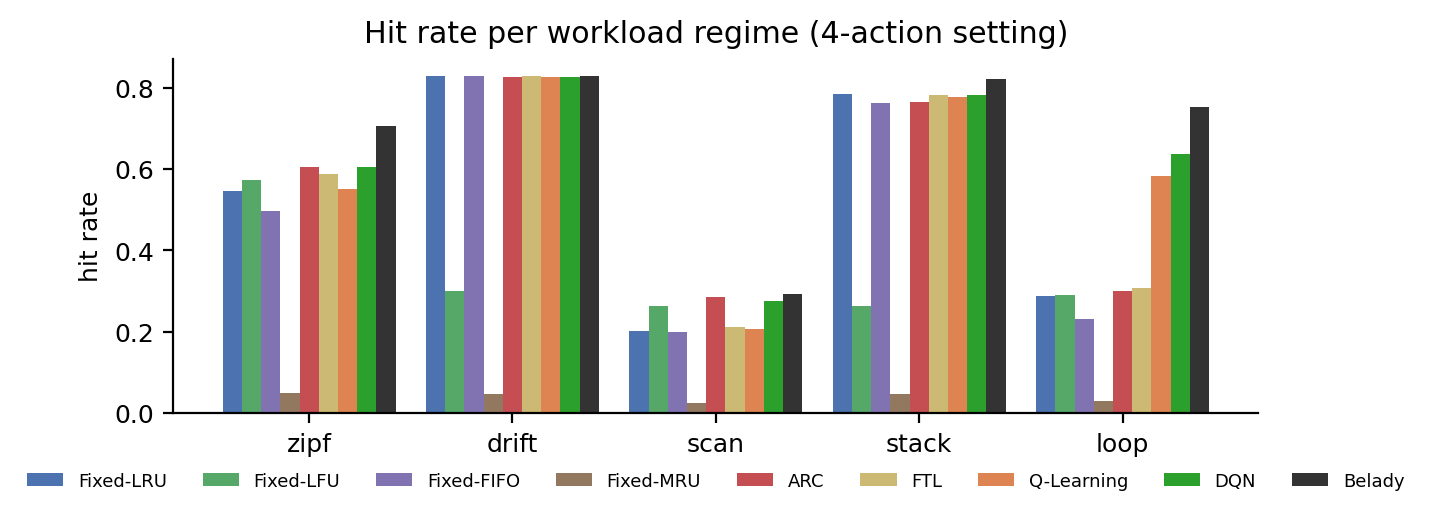
\includegraphics[width=\columnwidth]{figures/per_regime_a4.png}
  \caption{Hit rate per workload regime (4-action setting).}
  \label{fig:regime}
\end{figure}

\begin{figure}[t]
  \centering
  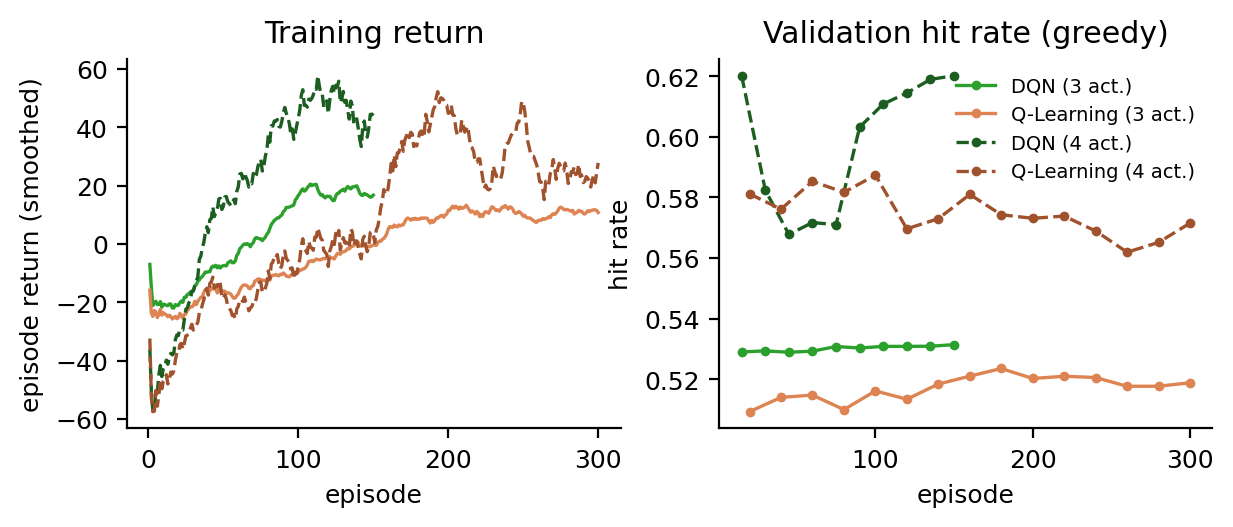
\includegraphics[width=\columnwidth]{figures/training_curves.png}
  \caption{Training return ($\epsilon$-greedy, smoothed) and greedy hit rate on the 8 validation
  traces. Return rises mostly as $\epsilon$ decays; DQN's greedy policy is near its final quality
  by the first evaluation (episode 15).}
  \label{fig:training}
\end{figure}

\textbf{Overall (Table~\ref{tab:main}).} Per-trace paired comparisons (Wilcoxon signed-rank, 20
traces): with 3 actions DQN beats ARC by $+0.38$\,pp (95\% CI $[0.19,0.57]$, 18/20 traces,
$p{=}8.5{\times}10^{-4}$), FTL by $+1.77$\,pp and LRU by $+2.79$\,pp (20/20 each).
Tabular Q-learning beats FTL and LRU but trails ARC by $0.32$\,pp ($p{=}0.04$). With MRU, DQN
leads ARC by $+6.46$\,pp (19/20, $p{<}10^{-5}$) and lowers AMAT by 19.2\% versus LRU.

\textbf{Where the gain comes from (Fig.~\ref{fig:regime},~\ref{fig:timeline}).} In the 3-action
setting DQN uses aged LFU in zipf, scan and loop phases (94--99\% of windows) and LRU/FIFO in drift
and stack, which mainly helps on scans (0.278 vs.\ 0.201 for LRU) and zipf (0.608 vs.\ 0.547).
The large +MRU gain is concentrated in loops (0.636 vs.\ 0.299 for ARC; Belady 0.753): the agent
first lets LRU/LFU refill the cache with loop blocks, then switches to MRU to pin them. Fixed MRU
fails (4.3\%) because it pins stale blocks from earlier phases, so this \emph{sequence} is
something no single static policy achieves. Switching \emph{within} phases is also why DQN beats
Phase-Oracle (57.50 vs.\ 56.79 with 3 actions, 63.58 vs.\ 57.22 with 4), so Phase-Oracle is
\emph{not} an upper bound on switching policies.

\textbf{Recovery and transfer.} Right after a phase change all methods dip (first window: DQN
0.48, LRU 0.50, ARC 0.47); DQN has the best 10-window post-change mean among online methods (Table~\ref{tab:main}).
Evaluated without retraining at $C{=}200$, DQN remains best among online methods (57.6\% vs.\ ARC
57.0\%); at $C{=}50$ it falls slightly behind ARC (56.2\% vs.\ 56.5\%).

\textbf{Limitations.} Traces are synthetic; agents are trained from a single seed; four full-size shadow caches add $4\times$ the cache's metadata
(set sampling as in DIP~\cite{qureshi2007dip} would reduce this); the end of a trace is a time limit
but is bootstrapped as terminal; and none of our baselines defends against loops (loop-resistant
LIRS~\cite{jiang2002lirs} was not evaluated), so the +MRU gain partly reflects the larger action set.

\section{Conclusion}
Learning \emph{when} to switch among simple eviction rules, rather than learning a new rule,
gives a cheap (one MLP call per 100 requests), interpretable policy. It is consistently better
than ARC and, with MRU available, recovers 64\% of the gap between LRU and Belady's optimum.

{\footnotesize
\setlength{\itemsep}{0pt}
\bibliographystyle{IEEEtran}
\bibliography{references}}

\end{document}
